% Options for packages loaded elsewhere
\PassOptionsToPackage{unicode}{hyperref}
\PassOptionsToPackage{hyphens}{url}
\PassOptionsToPackage{dvipsnames,svgnames,x11names}{xcolor}
%
\documentclass[
  letterpaper,
  DIV=11,
  numbers=noendperiod]{scrartcl}

\usepackage{amsmath,amssymb}
\usepackage{iftex}
\ifPDFTeX
  \usepackage[T1]{fontenc}
  \usepackage[utf8]{inputenc}
  \usepackage{textcomp} % provide euro and other symbols
\else % if luatex or xetex
  \usepackage{unicode-math}
  \defaultfontfeatures{Scale=MatchLowercase}
  \defaultfontfeatures[\rmfamily]{Ligatures=TeX,Scale=1}
\fi
\usepackage{lmodern}
\ifPDFTeX\else  
    % xetex/luatex font selection
\fi
% Use upquote if available, for straight quotes in verbatim environments
\IfFileExists{upquote.sty}{\usepackage{upquote}}{}
\IfFileExists{microtype.sty}{% use microtype if available
  \usepackage[]{microtype}
  \UseMicrotypeSet[protrusion]{basicmath} % disable protrusion for tt fonts
}{}
\makeatletter
\@ifundefined{KOMAClassName}{% if non-KOMA class
  \IfFileExists{parskip.sty}{%
    \usepackage{parskip}
  }{% else
    \setlength{\parindent}{0pt}
    \setlength{\parskip}{6pt plus 2pt minus 1pt}}
}{% if KOMA class
  \KOMAoptions{parskip=half}}
\makeatother
\usepackage{xcolor}
\setlength{\emergencystretch}{3em} % prevent overfull lines
\setcounter{secnumdepth}{-\maxdimen} % remove section numbering
% Make \paragraph and \subparagraph free-standing
\ifx\paragraph\undefined\else
  \let\oldparagraph\paragraph
  \renewcommand{\paragraph}[1]{\oldparagraph{#1}\mbox{}}
\fi
\ifx\subparagraph\undefined\else
  \let\oldsubparagraph\subparagraph
  \renewcommand{\subparagraph}[1]{\oldsubparagraph{#1}\mbox{}}
\fi

\usepackage{color}
\usepackage{fancyvrb}
\newcommand{\VerbBar}{|}
\newcommand{\VERB}{\Verb[commandchars=\\\{\}]}
\DefineVerbatimEnvironment{Highlighting}{Verbatim}{commandchars=\\\{\}}
% Add ',fontsize=\small' for more characters per line
\usepackage{framed}
\definecolor{shadecolor}{RGB}{241,243,245}
\newenvironment{Shaded}{\begin{snugshade}}{\end{snugshade}}
\newcommand{\AlertTok}[1]{\textcolor[rgb]{0.68,0.00,0.00}{#1}}
\newcommand{\AnnotationTok}[1]{\textcolor[rgb]{0.37,0.37,0.37}{#1}}
\newcommand{\AttributeTok}[1]{\textcolor[rgb]{0.40,0.45,0.13}{#1}}
\newcommand{\BaseNTok}[1]{\textcolor[rgb]{0.68,0.00,0.00}{#1}}
\newcommand{\BuiltInTok}[1]{\textcolor[rgb]{0.00,0.23,0.31}{#1}}
\newcommand{\CharTok}[1]{\textcolor[rgb]{0.13,0.47,0.30}{#1}}
\newcommand{\CommentTok}[1]{\textcolor[rgb]{0.37,0.37,0.37}{#1}}
\newcommand{\CommentVarTok}[1]{\textcolor[rgb]{0.37,0.37,0.37}{\textit{#1}}}
\newcommand{\ConstantTok}[1]{\textcolor[rgb]{0.56,0.35,0.01}{#1}}
\newcommand{\ControlFlowTok}[1]{\textcolor[rgb]{0.00,0.23,0.31}{#1}}
\newcommand{\DataTypeTok}[1]{\textcolor[rgb]{0.68,0.00,0.00}{#1}}
\newcommand{\DecValTok}[1]{\textcolor[rgb]{0.68,0.00,0.00}{#1}}
\newcommand{\DocumentationTok}[1]{\textcolor[rgb]{0.37,0.37,0.37}{\textit{#1}}}
\newcommand{\ErrorTok}[1]{\textcolor[rgb]{0.68,0.00,0.00}{#1}}
\newcommand{\ExtensionTok}[1]{\textcolor[rgb]{0.00,0.23,0.31}{#1}}
\newcommand{\FloatTok}[1]{\textcolor[rgb]{0.68,0.00,0.00}{#1}}
\newcommand{\FunctionTok}[1]{\textcolor[rgb]{0.28,0.35,0.67}{#1}}
\newcommand{\ImportTok}[1]{\textcolor[rgb]{0.00,0.46,0.62}{#1}}
\newcommand{\InformationTok}[1]{\textcolor[rgb]{0.37,0.37,0.37}{#1}}
\newcommand{\KeywordTok}[1]{\textcolor[rgb]{0.00,0.23,0.31}{#1}}
\newcommand{\NormalTok}[1]{\textcolor[rgb]{0.00,0.23,0.31}{#1}}
\newcommand{\OperatorTok}[1]{\textcolor[rgb]{0.37,0.37,0.37}{#1}}
\newcommand{\OtherTok}[1]{\textcolor[rgb]{0.00,0.23,0.31}{#1}}
\newcommand{\PreprocessorTok}[1]{\textcolor[rgb]{0.68,0.00,0.00}{#1}}
\newcommand{\RegionMarkerTok}[1]{\textcolor[rgb]{0.00,0.23,0.31}{#1}}
\newcommand{\SpecialCharTok}[1]{\textcolor[rgb]{0.37,0.37,0.37}{#1}}
\newcommand{\SpecialStringTok}[1]{\textcolor[rgb]{0.13,0.47,0.30}{#1}}
\newcommand{\StringTok}[1]{\textcolor[rgb]{0.13,0.47,0.30}{#1}}
\newcommand{\VariableTok}[1]{\textcolor[rgb]{0.07,0.07,0.07}{#1}}
\newcommand{\VerbatimStringTok}[1]{\textcolor[rgb]{0.13,0.47,0.30}{#1}}
\newcommand{\WarningTok}[1]{\textcolor[rgb]{0.37,0.37,0.37}{\textit{#1}}}

\providecommand{\tightlist}{%
  \setlength{\itemsep}{0pt}\setlength{\parskip}{0pt}}\usepackage{longtable,booktabs,array}
\usepackage{calc} % for calculating minipage widths
% Correct order of tables after \paragraph or \subparagraph
\usepackage{etoolbox}
\makeatletter
\patchcmd\longtable{\par}{\if@noskipsec\mbox{}\fi\par}{}{}
\makeatother
% Allow footnotes in longtable head/foot
\IfFileExists{footnotehyper.sty}{\usepackage{footnotehyper}}{\usepackage{footnote}}
\makesavenoteenv{longtable}
\usepackage{graphicx}
\makeatletter
\def\maxwidth{\ifdim\Gin@nat@width>\linewidth\linewidth\else\Gin@nat@width\fi}
\def\maxheight{\ifdim\Gin@nat@height>\textheight\textheight\else\Gin@nat@height\fi}
\makeatother
% Scale images if necessary, so that they will not overflow the page
% margins by default, and it is still possible to overwrite the defaults
% using explicit options in \includegraphics[width, height, ...]{}
\setkeys{Gin}{width=\maxwidth,height=\maxheight,keepaspectratio}
% Set default figure placement to htbp
\makeatletter
\def\fps@figure{htbp}
\makeatother

\KOMAoption{captions}{tableheading}
\makeatletter
\makeatother
\makeatletter
\makeatother
\makeatletter
\@ifpackageloaded{caption}{}{\usepackage{caption}}
\AtBeginDocument{%
\ifdefined\contentsname
  \renewcommand*\contentsname{Table of contents}
\else
  \newcommand\contentsname{Table of contents}
\fi
\ifdefined\listfigurename
  \renewcommand*\listfigurename{List of Figures}
\else
  \newcommand\listfigurename{List of Figures}
\fi
\ifdefined\listtablename
  \renewcommand*\listtablename{List of Tables}
\else
  \newcommand\listtablename{List of Tables}
\fi
\ifdefined\figurename
  \renewcommand*\figurename{Figure}
\else
  \newcommand\figurename{Figure}
\fi
\ifdefined\tablename
  \renewcommand*\tablename{Table}
\else
  \newcommand\tablename{Table}
\fi
}
\@ifpackageloaded{float}{}{\usepackage{float}}
\floatstyle{ruled}
\@ifundefined{c@chapter}{\newfloat{codelisting}{h}{lop}}{\newfloat{codelisting}{h}{lop}[chapter]}
\floatname{codelisting}{Listing}
\newcommand*\listoflistings{\listof{codelisting}{List of Listings}}
\makeatother
\makeatletter
\@ifpackageloaded{caption}{}{\usepackage{caption}}
\@ifpackageloaded{subcaption}{}{\usepackage{subcaption}}
\makeatother
\makeatletter
\@ifpackageloaded{tcolorbox}{}{\usepackage[skins,breakable]{tcolorbox}}
\makeatother
\makeatletter
\@ifundefined{shadecolor}{\definecolor{shadecolor}{rgb}{.97, .97, .97}}
\makeatother
\makeatletter
\makeatother
\makeatletter
\makeatother
\ifLuaTeX
  \usepackage{selnolig}  % disable illegal ligatures
\fi
\IfFileExists{bookmark.sty}{\usepackage{bookmark}}{\usepackage{hyperref}}
\IfFileExists{xurl.sty}{\usepackage{xurl}}{} % add URL line breaks if available
\urlstyle{same} % disable monospaced font for URLs
\hypersetup{
  pdftitle={Working with text using stringr},
  pdfauthor={Violet Ross and Emily Malcolm-White},
  colorlinks=true,
  linkcolor={blue},
  filecolor={Maroon},
  citecolor={Blue},
  urlcolor={Blue},
  pdfcreator={LaTeX via pandoc}}

\title{Working with text using \texttt{stringr}}
\author{Violet Ross and Emily Malcolm-White}
\date{}

\begin{document}
\maketitle
\ifdefined\Shaded\renewenvironment{Shaded}{\begin{tcolorbox}[breakable, boxrule=0pt, interior hidden, sharp corners, borderline west={3pt}{0pt}{shadecolor}, frame hidden, enhanced]}{\end{tcolorbox}}\fi


\includegraphics[width=0.3\textwidth,height=\textheight]{118_stringr_files/mediabag/logo.png}

\begin{figure}

{\centering 
\includegraphics[width=0.5\textwidth,height=\textheight]{118_stringr_files/mediabag/6bbcc35c-1863-49df-8.png}

}

\caption{artwork by @allisonhorst}

\end{figure}

\hypertarget{a-few-basics}{%
\section{A few basics}\label{a-few-basics}}

\textbf{What is a string?}

\begin{itemize}
\tightlist
\item
  datatype we use to represent text
\item
  use '' ''
\end{itemize}

\textbf{Examples of strings:}

\begin{itemize}
\tightlist
\item
  ``Hello world''
\item
  ``5678''
\item
  ``blah blah blah''
\end{itemize}

** NOT a string:**

\begin{itemize}
\tightlist
\item
  5678
\end{itemize}

\hypertarget{using-stringr}{%
\section{\texorpdfstring{Using
\texttt{stringr}}{Using stringr}}\label{using-stringr}}

\href{https://stringr.tidyverse.org/}{\texttt{stringr}} is a package
containing a bunch of functions that help us work with strings. We'll
discuss how to detect, remove, extract, and count
words/characters/phrases from a string. We'll also talk about how to
slice a string to get only the parts (aka the substrings) of it that you
want.

\href{https://evoldyn.gitlab.io/evomics-2018/ref-sheets/R_strings.pdf}{\textbf{\texttt{stringr}
cheat sheet}}

\texttt{stringr} is contained within the \texttt{tidyverse} package.

\begin{Shaded}
\begin{Highlighting}[]
\FunctionTok{library}\NormalTok{(tidyverse)}
\end{Highlighting}
\end{Shaded}

\textbf{I'm registering for classes this Spring and am trying to decide
what to take.} Let's look at the course catalog!

Read in the courses data.

\begin{Shaded}
\begin{Highlighting}[]
\NormalTok{courses }\OtherTok{\textless{}{-}} \FunctionTok{read\_csv}\NormalTok{(}\StringTok{"data/Fall23courses.csv"}\NormalTok{)}
\end{Highlighting}
\end{Shaded}

\hypertarget{str_detect}{%
\subsection{\texorpdfstring{\texttt{str\_detect}}{str\_detect}}\label{str_detect}}

\begin{figure}

{\centering 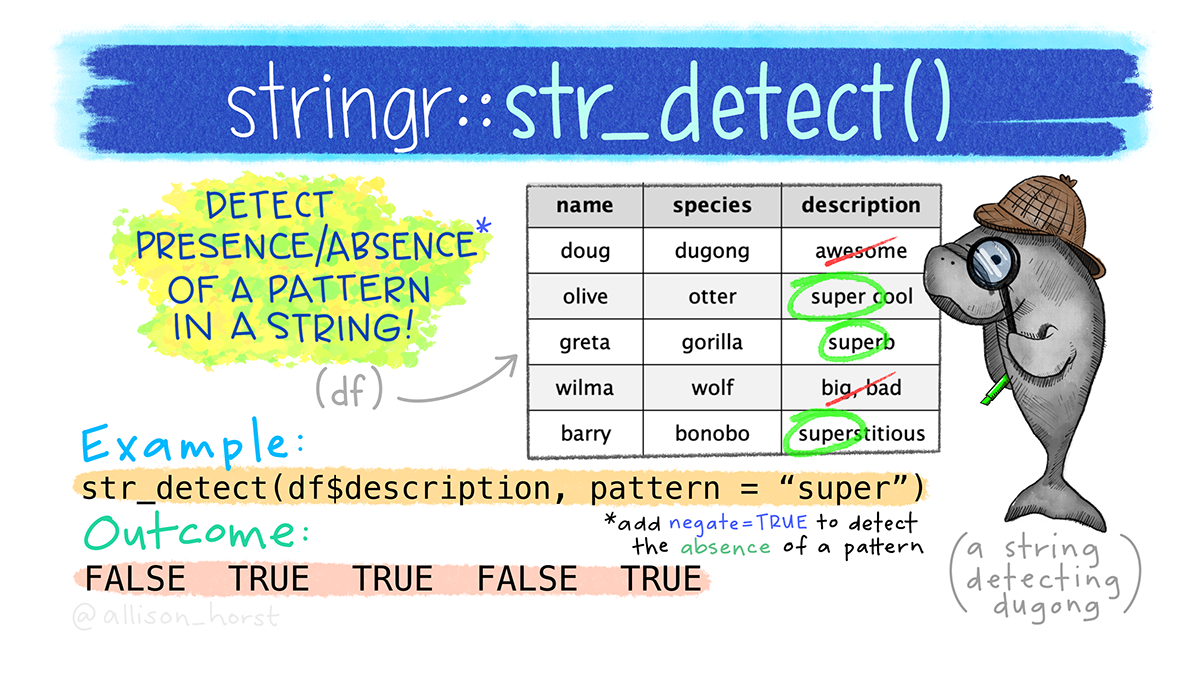
\includegraphics{118_stringr_files/mediabag/813129dc-25e9-4ea3-9.png}

}

\caption{artwork by @allisonhorst}

\end{figure}

\textbf{inputs}: - string - pattern

\textbf{output}: - TRUE/FALSE

little example:

\begin{Shaded}
\begin{Highlighting}[]
\FunctionTok{str\_detect}\NormalTok{(}\StringTok{"Welcome to data science, look at this cool data"}\NormalTok{, }\StringTok{"data"}\NormalTok{)}
\end{Highlighting}
\end{Shaded}

\begin{verbatim}
[1] TRUE
\end{verbatim}

\begin{Shaded}
\begin{Highlighting}[]
\FunctionTok{str\_detect}\NormalTok{(}\StringTok{"Welcome to data science, look at this cool data"}\NormalTok{, }\StringTok{"pineapple"}\NormalTok{)}
\end{Highlighting}
\end{Shaded}

\begin{verbatim}
[1] FALSE
\end{verbatim}

I only want to take classes in Warner!

\begin{Shaded}
\begin{Highlighting}[]
\NormalTok{courses }\SpecialCharTok{\%\textgreater{}\%} 
  \FunctionTok{filter}\NormalTok{(}\FunctionTok{str\_detect}\NormalTok{(location, }\StringTok{"WNS"}\NormalTok{))}
\end{Highlighting}
\end{Shaded}

\begin{verbatim}
# A tibble: 45 x 9
   titles      distros department time  location professor description courseNum
   <chr>       <chr>   <chr>      <chr> <chr>    <chr>     <chr>       <chr>    
 1 Gothic and~ AMR HI~ Program i~ 2:15~ "Warner~ Michael ~ "\nThis co~ AMST0225~
 2 Education ~ AMR SOC Program i~ 2:15~ "Warner~ Melissa ~ "\nWhat ar~ BLST0115~
 3 Economic S~ DED     Economics  2:15~ "Warner~ Amanda G~ "\nAn intr~ ECON0111~
 4 Introducto~ SOC     Economics  9:45~ "Warner~ Raphaell~ "\nAn intr~ ECON0150~
 5 Introducto~ SOC     Economics  11:1~ "Warner~ Raphaell~ "\nAn intr~ ECON0150~
 6 Introducto~ SOC     Economics  8:15~ "Warner~ Will Pyle "\nAn intr~ ECON0155~
 7 Introducto~ SOC     Economics  9:45~ "Warner~ Will Pyle "\nAn intr~ ECON0155~
 8 Microecono~ <NA>    Economics  12:4~ "Warner~ <NA>      "\nMicroec~ ECON0255~
 9 Microecono~ <NA>    Economics  2:15~ "Warner~ <NA>      "\nMicroec~ ECON0255~
10 Federal Re~ AMR DED Economics  1:30~ "Warner~ Erin Wol~ "\nIn this~ ECON0360~
# i 35 more rows
# i 1 more variable: meet <chr>
\end{verbatim}

Suppose I don't want any classes on Friday. Let's use
\texttt{str\_detect} to find our options.

\begin{Shaded}
\begin{Highlighting}[]
\NormalTok{notFriday }\OtherTok{\textless{}{-}}\NormalTok{ courses }\SpecialCharTok{\%\textgreater{}\%} 
  \FunctionTok{filter}\NormalTok{(}\SpecialCharTok{!}\FunctionTok{str\_detect}\NormalTok{(meet, }\StringTok{"Friday"}\NormalTok{))}
\end{Highlighting}
\end{Shaded}

Perhaps I'm interested in immigration.

The \texttt{regex} function is used to write regular expressions in R.
Regular expressions are helpful if you want to search for a pattern
rather than a specific word or phrase.

For now, we will only use regex to ignore capitalization.

If you're interested in using regular expressions at some point, this
\href{https://cheatography.com/davechild/cheat-sheets/regular-expressions/}{regex
cheat sheet} will be super helpful.

\begin{Shaded}
\begin{Highlighting}[]
\NormalTok{immigrationclasses }\OtherTok{\textless{}{-}}\NormalTok{ courses }\SpecialCharTok{\%\textgreater{}\%} 
  \FunctionTok{filter}\NormalTok{(}\FunctionTok{str\_detect}\NormalTok{(description, }\FunctionTok{regex}\NormalTok{(}\StringTok{"immigration"}\NormalTok{, }\AttributeTok{ignore\_case=}\ConstantTok{TRUE}\NormalTok{)))}

\NormalTok{immigrationclasses}
\end{Highlighting}
\end{Shaded}

\begin{verbatim}
# A tibble: 10 x 9
   titles      distros department time  location professor description courseNum
   <chr>       <chr>   <chr>      <chr> <chr>    <chr>     <chr>       <chr>    
 1 Immigrant ~ AMR HIS Program i~ 11:1~ "Axinn ~ Rachael ~ "\nIn this~ AMST0175~
 2 Introducti~ EUR LN~ French     2:15~ "Le Cha~ William ~ "\nIn this~ FREN0230~
 3 Introducti~ CW EUR~ French     2:15~ "Le Cha~ William ~ "\nIn this~ FREN0230~
 4 The United~ AMR HIS History    9:45~ "Axinn ~ Joyce Mao "\nThis co~ HIST0206~
 5 Introducti~ CMP     Internati~ 12:4~ "Twilig~ Amit Pra~ "\nThis is~ IGST0101~
 6 An Introdu~ EUR LN~ Italian    9:45~ "Wright~ Thomas V~ "\nIntende~ ITAL0251~
 7 An Introdu~ EUR LN~ Italian    11:1~ "75 Sha~ Sandra C~ "\nIntende~ ITAL0251~
 8 Globalizat~ SOC     Political~ 2:15~ "Librar~ Orion Le~ "\nHow doe~ PSCI0314~
 9 City Polit~ <NA>    Political~ 11:1~ "LaForc~ Bert Joh~ "\nCities ~ PSCI0465~
10 Christiani~ AMR HI~ Religion   7:30~ "Librar~ James Ca~ "\nReligio~ RELI0398~
# i 1 more variable: meet <chr>
\end{verbatim}

\hypertarget{str_extract-and-str_remove}{%
\subsection{\texorpdfstring{\texttt{str\_extract} and
\texttt{str\_remove}}{str\_extract and str\_remove}}\label{str_extract-and-str_remove}}

\textbf{str\_extract inputs}: - string - pattern \textbf{str\_extract
output}: - the extracted pattern, if it appears in the the string

\textbf{str\_remove inputs}: - string - pattern \textbf{str\_extract
output}: - the string without the pattern, if it appears in the string

little example:

\begin{Shaded}
\begin{Highlighting}[]
\FunctionTok{str\_extract}\NormalTok{(}\StringTok{"Welcome to data science, look at this cool data"}\NormalTok{, }\StringTok{"data"}\NormalTok{)}
\end{Highlighting}
\end{Shaded}

\begin{verbatim}
[1] "data"
\end{verbatim}

\begin{Shaded}
\begin{Highlighting}[]
\FunctionTok{str\_extract\_all}\NormalTok{(}\StringTok{"Welcome to data science, look at this cool data"}\NormalTok{, }\StringTok{"data"}\NormalTok{)}
\end{Highlighting}
\end{Shaded}

\begin{verbatim}
[[1]]
[1] "data" "data"
\end{verbatim}

\begin{Shaded}
\begin{Highlighting}[]
\FunctionTok{str\_remove}\NormalTok{(}\StringTok{"Welcome to data science, look at this cool data"}\NormalTok{, }\StringTok{"data"}\NormalTok{)}
\end{Highlighting}
\end{Shaded}

\begin{verbatim}
[1] "Welcome to  science, look at this cool data"
\end{verbatim}

\begin{Shaded}
\begin{Highlighting}[]
\FunctionTok{str\_remove\_all}\NormalTok{(}\StringTok{"Welcome to data science, look at this cool data"}\NormalTok{, }\StringTok{"data"}\NormalTok{)}
\end{Highlighting}
\end{Shaded}

\begin{verbatim}
[1] "Welcome to  science, look at this cool "
\end{verbatim}

CW is part of the distribution requirement column. I want CW to be its
own column.

\begin{Shaded}
\begin{Highlighting}[]
\NormalTok{courses }\SpecialCharTok{\%\textgreater{}\%} 
  \FunctionTok{mutate}\NormalTok{(}\AttributeTok{CW =} \FunctionTok{str\_extract}\NormalTok{(distros, }\StringTok{"CW"}\NormalTok{)) }\SpecialCharTok{\%\textgreater{}\%} 
  \FunctionTok{mutate}\NormalTok{(}\AttributeTok{distros =} \FunctionTok{str\_remove}\NormalTok{(distros, }\StringTok{"CW"}\NormalTok{))}
\end{Highlighting}
\end{Shaded}

\begin{verbatim}
# A tibble: 586 x 10
   titles      distros department time  location professor description courseNum
   <chr>       <chr>   <chr>      <chr> <chr>    <chr>     <chr>       <chr>    
 1 Introducti~ AMR CMP Program i~ 12:4~ "Axinn ~ Roberto ~ "\nIn this~ AMST0101~
 2 Immigrant ~ AMR HIS Program i~ 11:1~ "Axinn ~ Rachael ~ "\nIn this~ AMST0175~
 3 American L~ AMR LIT Program i~ 11:1~ "Axinn ~ Ellery F~ "\nA study~ AMST0209~
 4 Introducti~ AMR HI~ Program i~ 1:30~ "Twilig~ Roberto ~ "\nIn this~ AMST0213~
 5 Gothic and~ AMR HI~ Program i~ 2:15~ "Warner~ Michael ~ "\nThis co~ AMST0225~
 6 American C~ AMR HIS Program i~ 9:45~ "Axinn ~ Holly Al~ "\nFor man~ AMST0234~
 7 Constructi~ AMR ART Program i~ 1:30~ "Ross C~ Deb Evans "\n“Democr~ AMST0251~
 8 African Am~ AMR LIT Program i~ 9:45~ "Axinn ~ William ~ "\nThis co~ AMST0252~
 9 American D~ AMR HI~ Program i~ 11:1~ "Axinn ~ Susan Bu~ "\nIn this~ AMST0260~
10 Chicagoland AMR HIS Program i~ 11:1~ "Giffor~ Jim Ralp~ "\nIn this~ AMST0264~
# i 576 more rows
# i 2 more variables: meet <chr>, CW <chr>
\end{verbatim}

\hypertarget{str_sub}{%
\subsection{\texorpdfstring{\texttt{str\_sub}}{str\_sub}}\label{str_sub}}

\textbf{str\_sub inputs}: - string\\
- starting character - ending character \textbf{str\_sub output}: -
string with only the characters between the start and the end

little example:

\begin{Shaded}
\begin{Highlighting}[]
\FunctionTok{str\_sub}\NormalTok{(}\StringTok{"Welcome to data science, look at this cool data"}\NormalTok{, }\AttributeTok{start=}\DecValTok{12}\NormalTok{, }\AttributeTok{end=}\DecValTok{23}\NormalTok{) }
\end{Highlighting}
\end{Shaded}

\begin{verbatim}
[1] "data science"
\end{verbatim}

Bounds are inclusive!

Maybe I only want 200 level math classes.

\begin{itemize}
\tightlist
\item
  First we filter for just math classes.
\item
  Then we can create a new column called \texttt{level} that contains
  only the sixth character from the \texttt{courses} column.
\end{itemize}

We call this a \textbf{substring}, hence the function \texttt{str\_sub}.

\begin{Shaded}
\begin{Highlighting}[]
\NormalTok{MathClasses }\OtherTok{\textless{}{-}}\NormalTok{ courses }\SpecialCharTok{\%\textgreater{}\%} 
  \FunctionTok{filter}\NormalTok{(department }\SpecialCharTok{==} \StringTok{"Mathematics"}\NormalTok{) }\SpecialCharTok{\%\textgreater{}\%} 
  \FunctionTok{mutate}\NormalTok{(}\AttributeTok{level=}\FunctionTok{str\_sub}\NormalTok{(courseNum, }\AttributeTok{start=}\DecValTok{6}\NormalTok{, }\AttributeTok{end=}\DecValTok{6}\NormalTok{)) }

\NormalTok{Math2Classes }\OtherTok{\textless{}{-}}\NormalTok{ MathClasses }\SpecialCharTok{\%\textgreater{}\%} 
  \FunctionTok{filter}\NormalTok{(level}\SpecialCharTok{==} \StringTok{"2"}\NormalTok{)}
\end{Highlighting}
\end{Shaded}

\hypertarget{str_count}{%
\subsection{\texorpdfstring{\texttt{str\_count}}{str\_count}}\label{str_count}}

\textbf{str\_count inputs}: - string\\
- pattern \textbf{str\_count output}: - a count of the number of times
the pattern appears in the string

little example:

\begin{Shaded}
\begin{Highlighting}[]
\FunctionTok{str\_count}\NormalTok{(}\StringTok{"Welcome to data science, look at this cool data"}\NormalTok{, }\StringTok{"data"}\NormalTok{)}
\end{Highlighting}
\end{Shaded}

\begin{verbatim}
[1] 2
\end{verbatim}

Maybe I only want my classes to meet twice a week.

\begin{Shaded}
\begin{Highlighting}[]
\NormalTok{courses }\OtherTok{\textless{}{-}}\NormalTok{ courses }\SpecialCharTok{\%\textgreater{}\%} 
  \FunctionTok{mutate}\NormalTok{(}\AttributeTok{dayCount =} \FunctionTok{str\_count}\NormalTok{(meet, }\StringTok{"day"}\NormalTok{))}

\CommentTok{\#what\textquotesingle{}s the maximum number of days a week a class meets?}
\FunctionTok{max}\NormalTok{(courses}\SpecialCharTok{$}\NormalTok{dayCount)}
\end{Highlighting}
\end{Shaded}

\begin{verbatim}
[1] 5
\end{verbatim}

\begin{Shaded}
\begin{Highlighting}[]
\CommentTok{\#what\textquotesingle{}s the mean number of days?}
\FunctionTok{mean}\NormalTok{(courses}\SpecialCharTok{$}\NormalTok{dayCount)}
\end{Highlighting}
\end{Shaded}

\begin{verbatim}
[1] 2.187713
\end{verbatim}

Let's visualize this data.

\begin{Shaded}
\begin{Highlighting}[]
\NormalTok{courses }\SpecialCharTok{\%\textgreater{}\%} 
  \FunctionTok{ggplot}\NormalTok{() }\SpecialCharTok{+} 
  \FunctionTok{geom\_bar}\NormalTok{(}\FunctionTok{aes}\NormalTok{(}\AttributeTok{x=}\NormalTok{dayCount), }\AttributeTok{fill=}\StringTok{"blue"}\NormalTok{) }\SpecialCharTok{+} 
  \FunctionTok{xlab}\NormalTok{(}\StringTok{"Number of Days Class Meets"}\NormalTok{) }\SpecialCharTok{+} 
  \FunctionTok{ylab}\NormalTok{(}\StringTok{"Number of Classes"}\NormalTok{) }\SpecialCharTok{+} 
  \FunctionTok{labs}\NormalTok{(}\AttributeTok{title=}\StringTok{"How many Days a Week do Classes at Middlebury Meet?"}\NormalTok{)}\SpecialCharTok{+}
  \FunctionTok{theme\_classic}\NormalTok{()}
\end{Highlighting}
\end{Shaded}

\begin{figure}[H]

{\centering 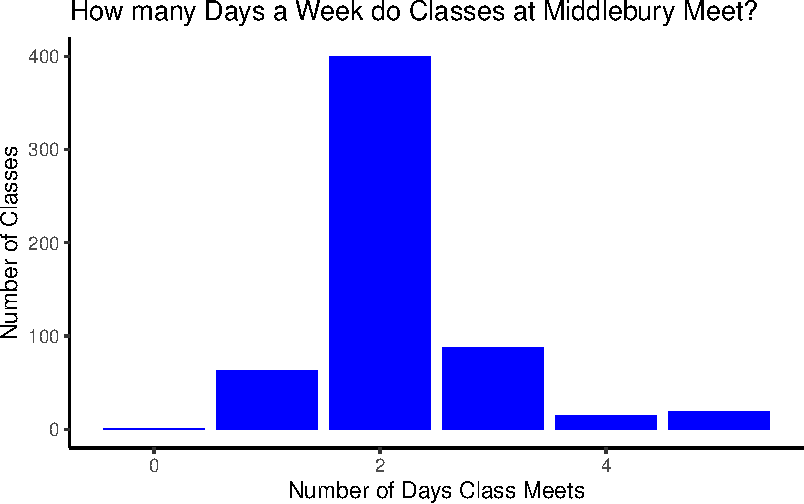
\includegraphics{118_stringr_files/figure-pdf/unnamed-chunk-14-1.pdf}

}

\end{figure}

\hypertarget{another-useful-function-str_squish}{%
\section{\texorpdfstring{Another useful function
\texttt{str\_squish}}{Another useful function str\_squish}}\label{another-useful-function-str_squish}}

\texttt{str\_squish} is used to remove leading, trailing, and repeated
interior whitespaces from strings

\begin{figure}

{\centering 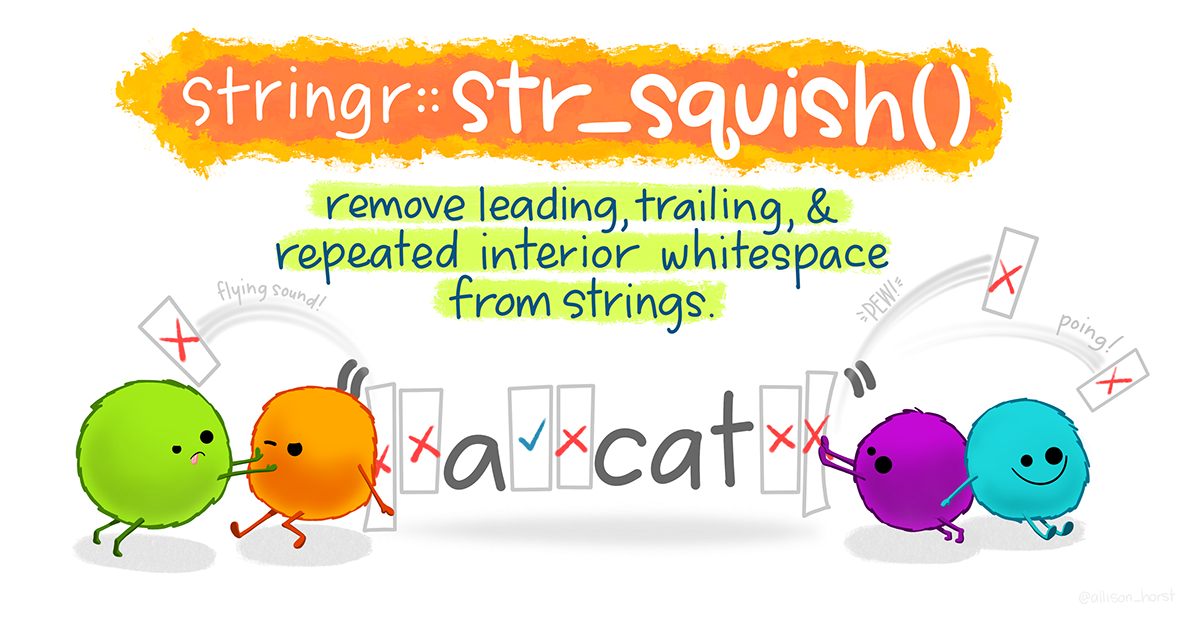
\includegraphics{118_stringr_files/mediabag/0e4df3af-8bca-4f5e-9.png}

}

\caption{artwork by @allisonhorst}

\end{figure}



\end{document}
